% ------------------------------------------------------------------------ %
% !TEX encoding = UTF-8
% !TEX TS-program = pdflatex
% !TEX root = ../Project.tex
% !TEX spellcheck = en-EN
% ------------------------------------------------------------------------ %
%
% ------------------------------------------------------------------------ %
% 	CHAPTER TITLE
% ------------------------------------------------------------------------ %
%
\chapter{Results}

\section{Test Rules}
For execution of the test some rules about the task performance are used.
Starting from the scoring method considered for the task success, the one used is the following:
\begin{itemize}
\item Complete success (without assistance) = 1
\item Partial success, or if assistance given = 0.5
\item Gives up or wrong answer = 0
\end{itemize}
For the determination of unsuccessful tasks, a task is considered unsuccessful if one of the following condition is matched:
\begin{itemize}
\item The user give up on trying to complete the task.
\item Three wrong paths, or three attempts from the start, but the user is free to persevere, even though the task is considered unsuccessful.
\item The cut-off time (threshold) is elapsed (for this test 4 minutes are chosen as cut-off time).
\end{itemize}
At last, action is considered an error if:
\begin{itemize}
\item The user enter incorrect data into a form field.
\item The user makes the wrong choice in a menu or drop-down list.
\item The user takes an incorrect sequence of actions.
\item The user fails to take a key action.
\end{itemize}
%
% ------------------------------------------------------------------------ %
%
\section{Documentation of the test}
All the data retrieved by the moderators and compiled by the users during the tests are presented below.

As reminder these ones are the tasks asked to the users:
\begin{itemize}
\item Task 1: You stumbled upon the website of ``The Big Family'', understand what is the scope of this association.
\item Task 2: You are helping a friend looking for services for disabled people near Certaldo. Identify the ones offered by the association.
\item Task 3: You want to write an email to have some more information about the association. Find the address.
\item Task 4: You need to contact someone working in the Pet Therapy service. Find a telephone number to call.
\item Task 5: You want to visit the association’s site nearest to your house. Find where it is.
\end{itemize}

\subsection{Task record sheet}
In the next page the data retrived by moderators during the test are presented, collected in the task record sheet. For every user and every task, the moderators observed:
\begin{itemize}
\item Task time
\item Task completion
\item Number of errors
\item Possible observation on the the behaviour of the user or comments
\end{itemize}

\newpage
\begin{center}
\makebox[\textwidth][c]{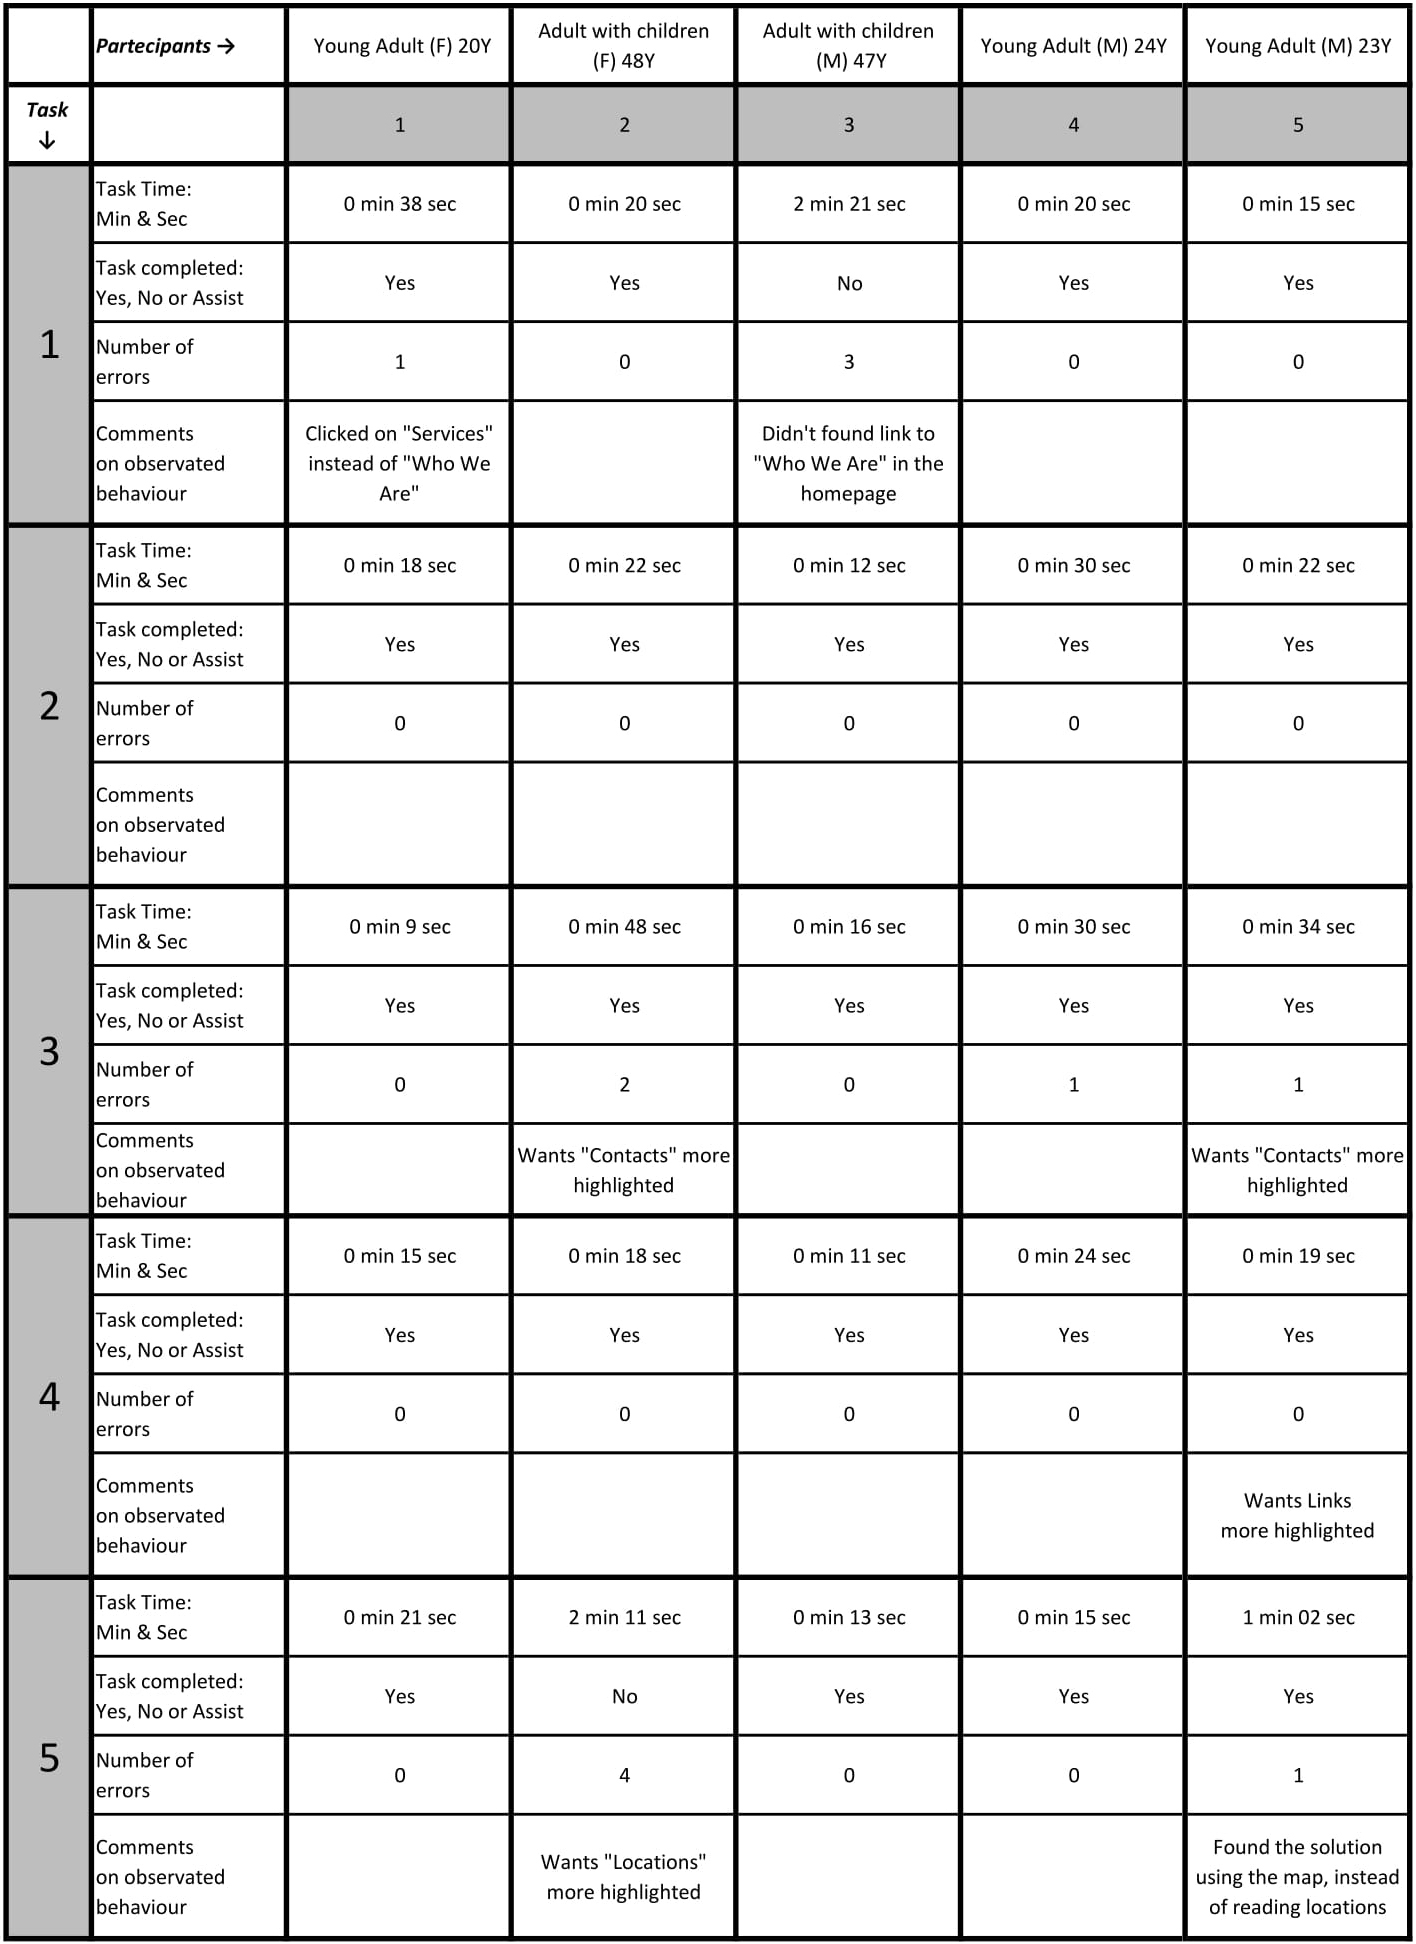
\includegraphics[width=1.11\textwidth]{Documents/taskrecord}}
\end{center}

\newpage
\subsection{Post test questionnaires}
These questionnaires are provided to the users after the execution of the test, in order to retrieve the overall feelings perceived by them regarding the tasks (like difficulty, disorientation...). The questionnaires are filled in by each one of the five people involved in the testing and are listed in the same order as in the task record sheet. The questionnaire used is the DEEP (Design oriented evaluation of perceived web usability), that is composed of questions about content, structure and navigation of the site.

\begin{center}
\makebox[\textwidth][c]{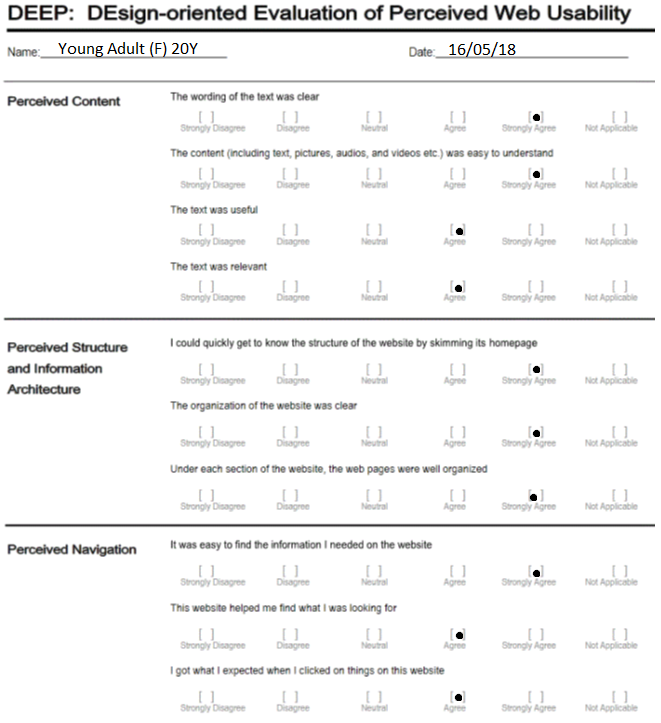
\includegraphics[width=1.09\textwidth]{Documents/post1}}
\newpage
\null
\vfill
\makebox[\textwidth][c]{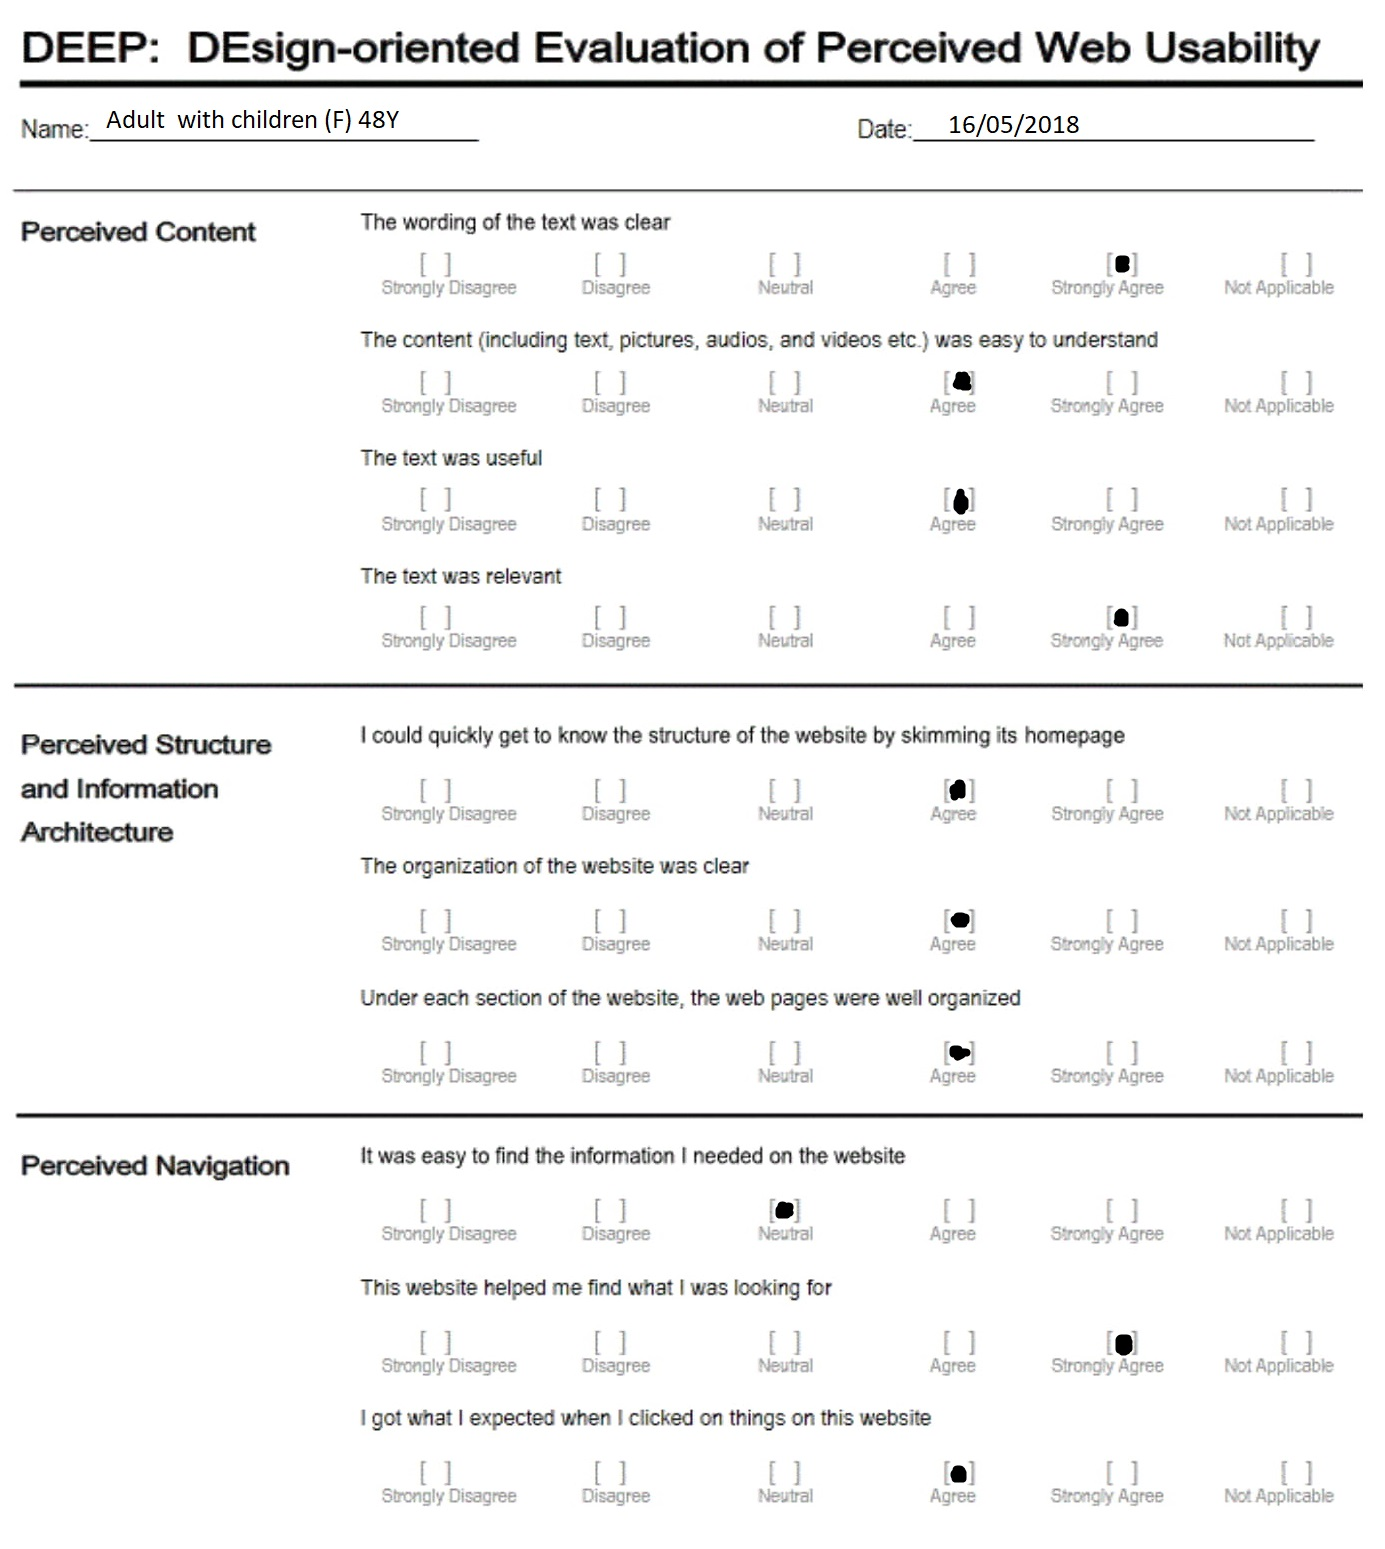
\includegraphics[width=1.09\textwidth]{Documents/post2}}
\vfill
\newpage
\null
\vfill
\makebox[\textwidth][c]{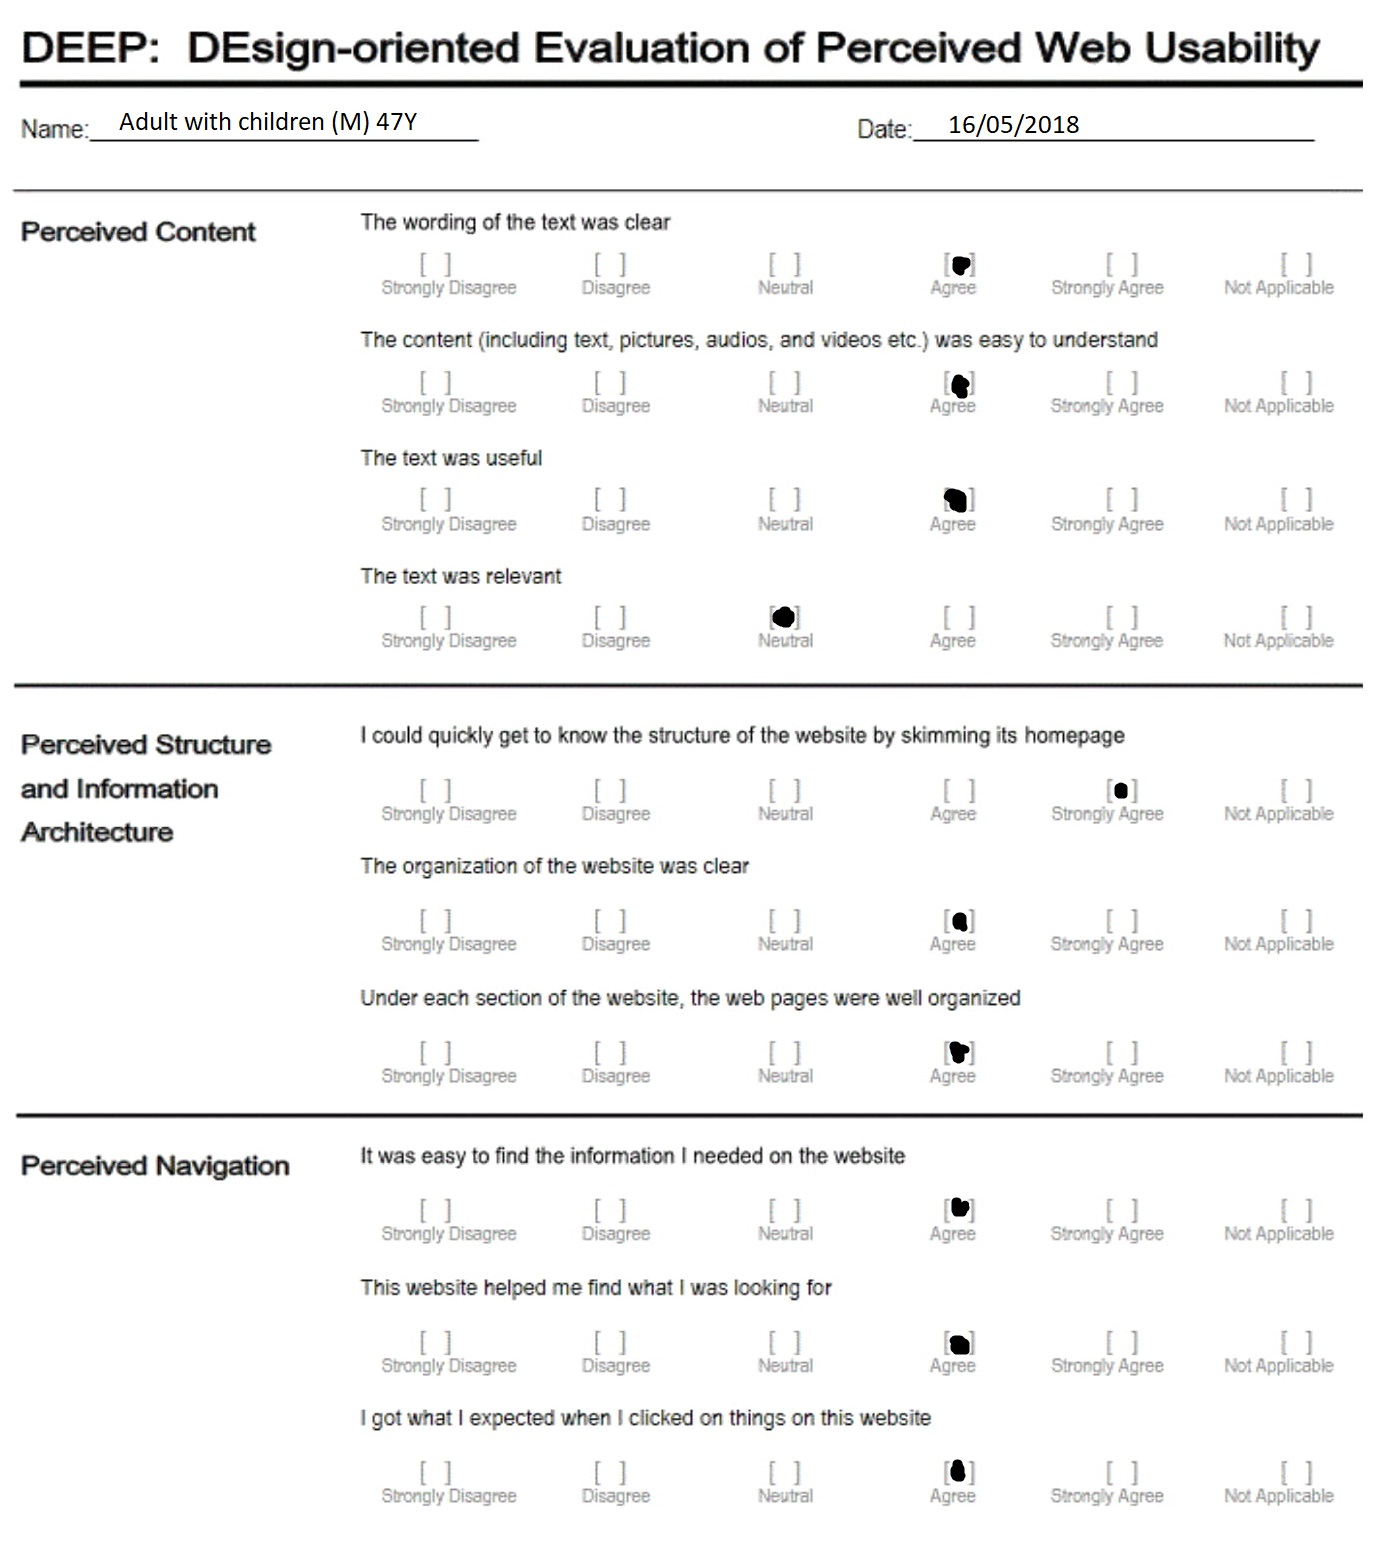
\includegraphics[width=1.09\textwidth]{Documents/post3}}
\vfill
\newpage
\null
\vfill
\makebox[\textwidth][c]{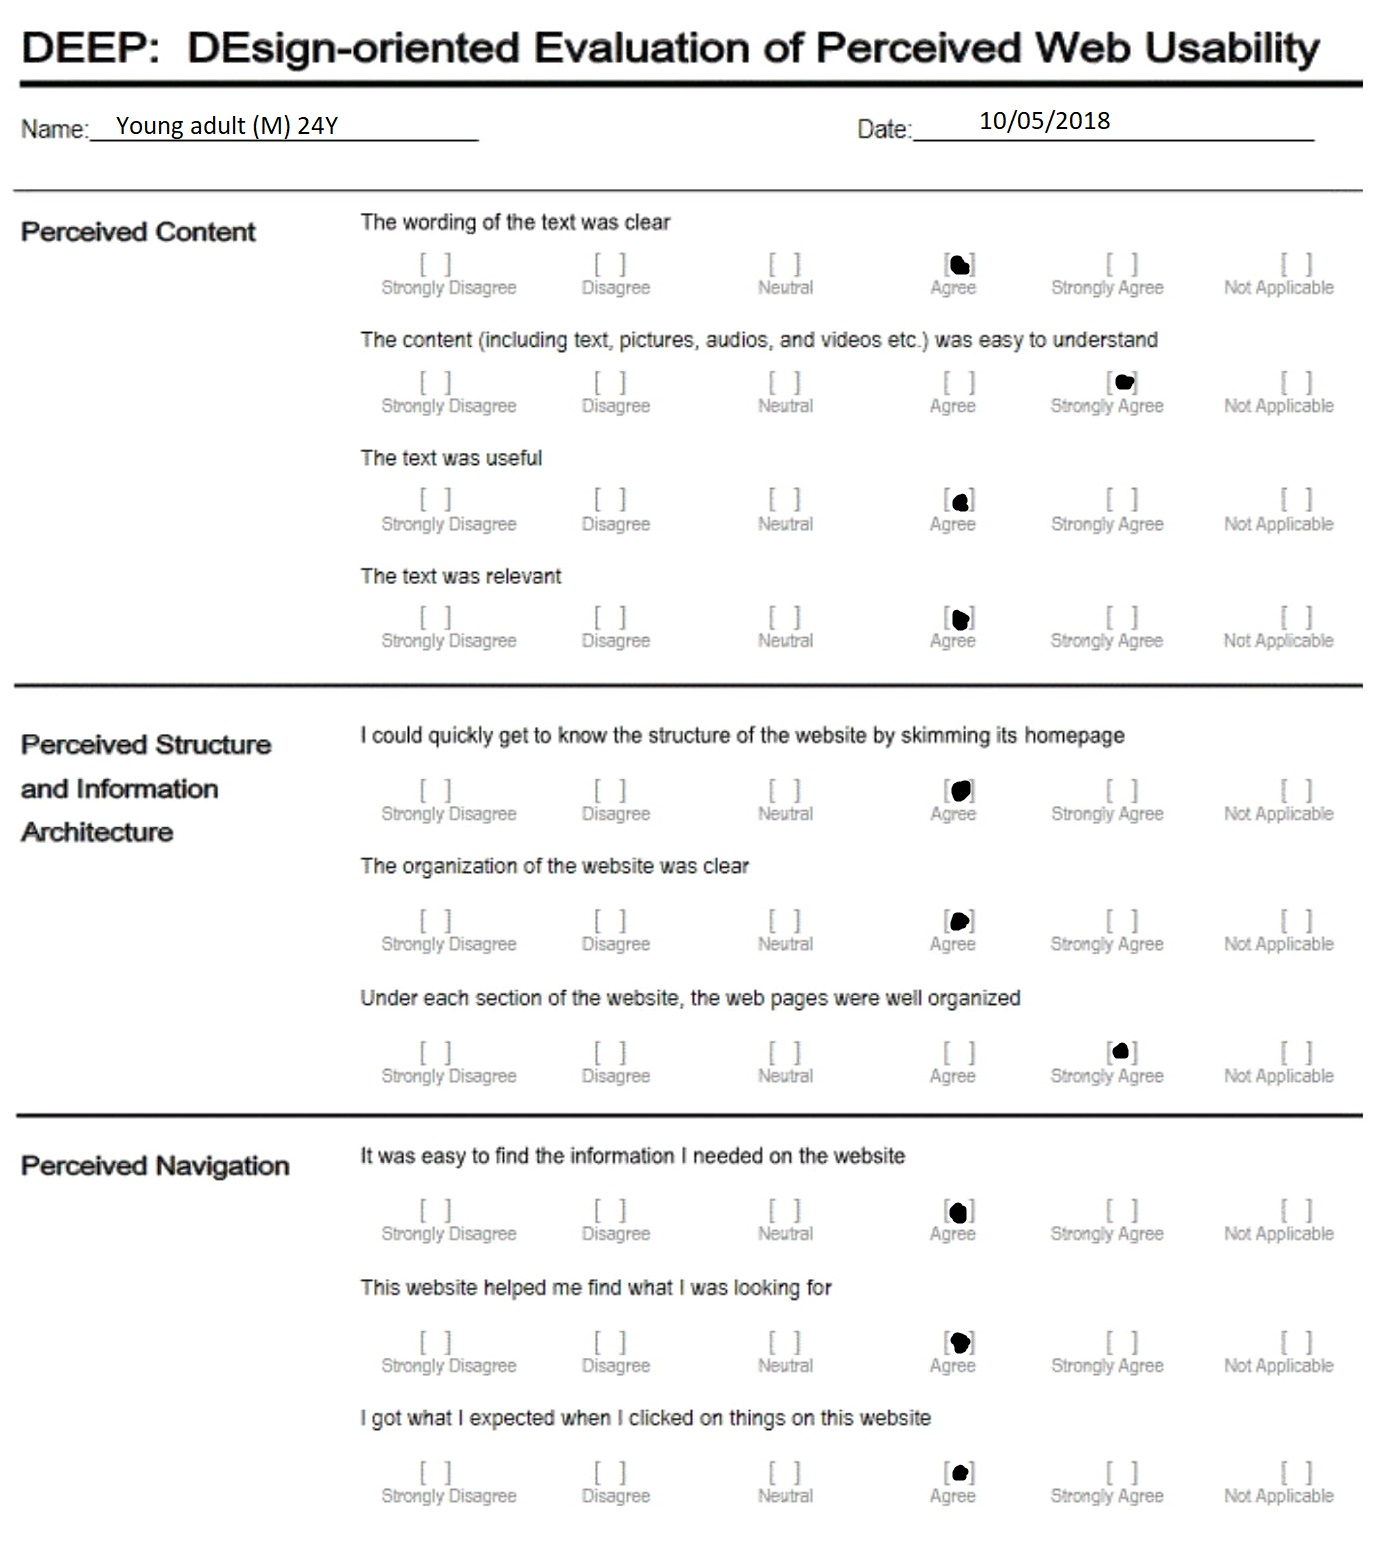
\includegraphics[width=1.09\textwidth]{Documents/post4}}
\vfill
\newpage
\null
\vfill
\makebox[\textwidth][c]{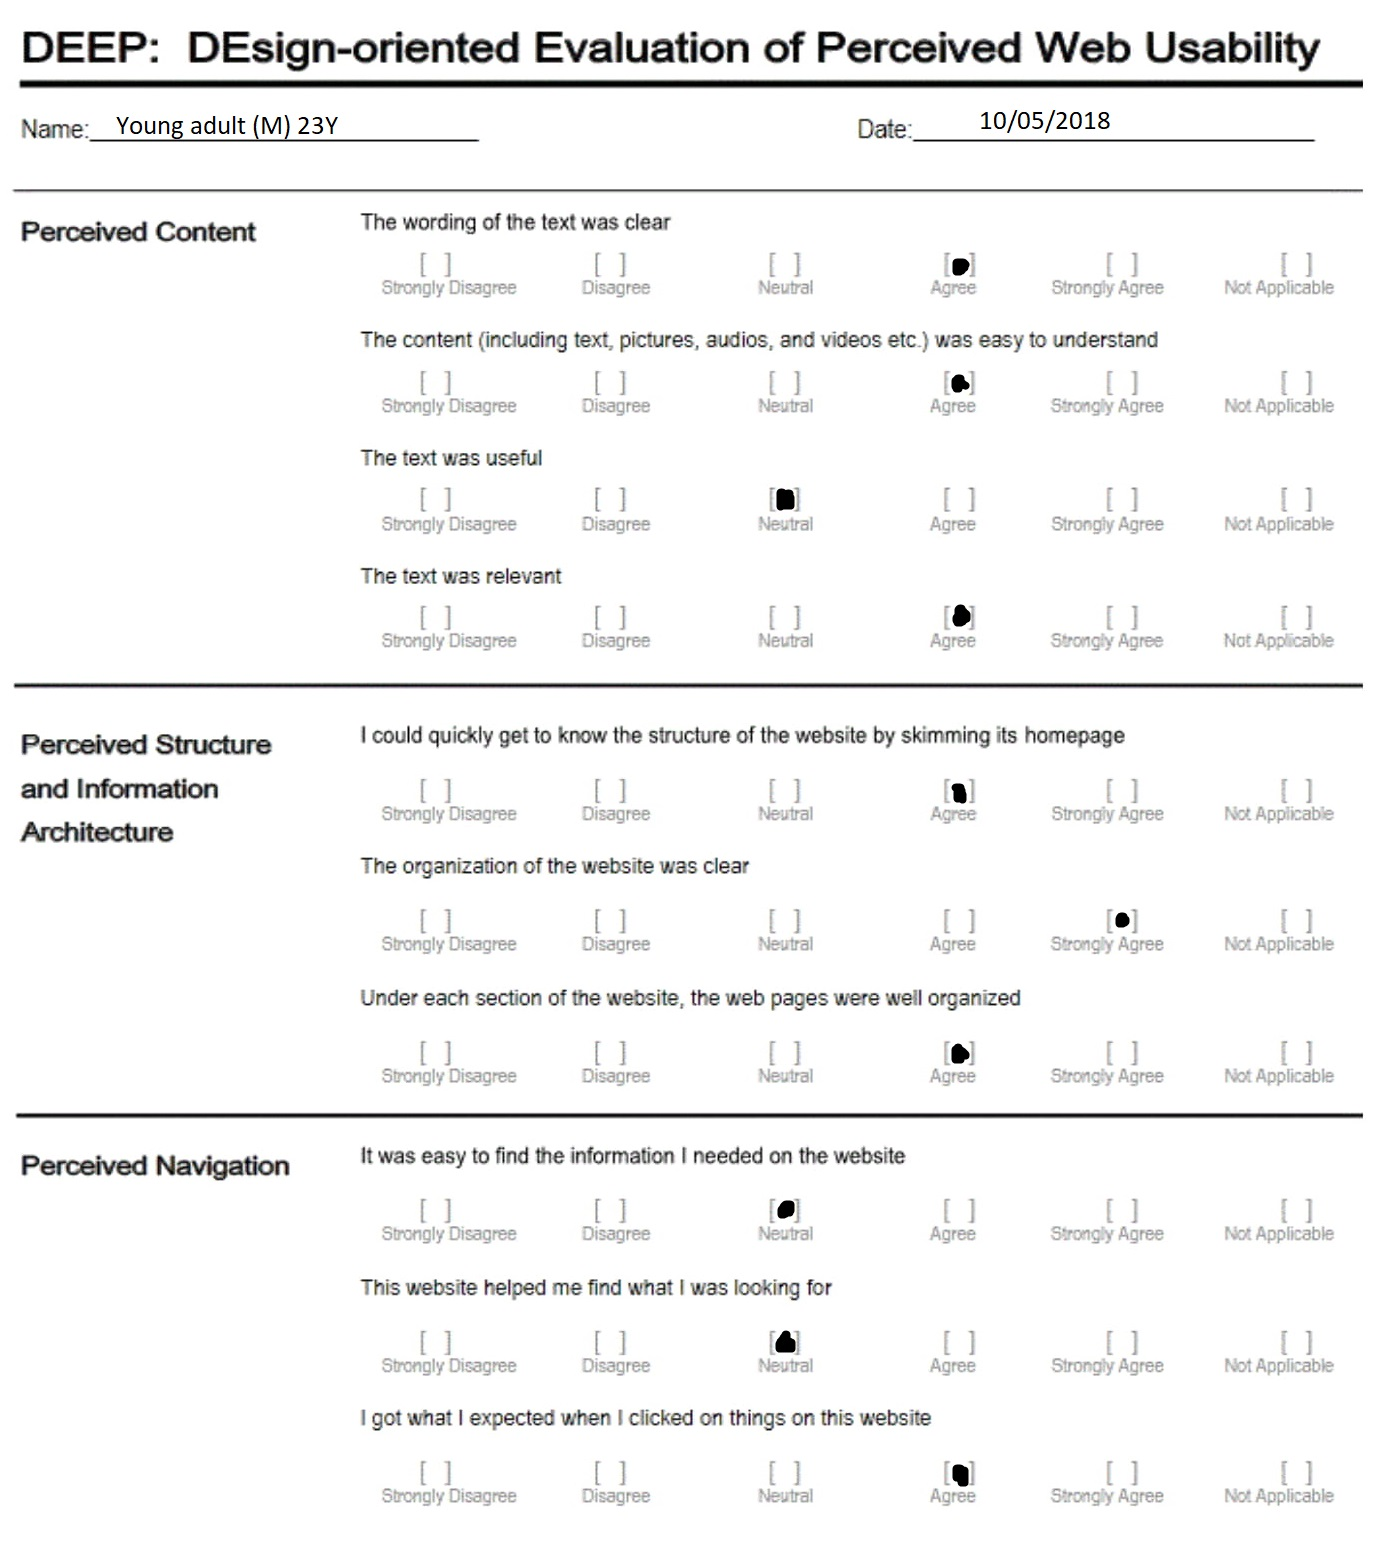
\includegraphics[width=1.09\textwidth]{Documents/post5}}
\vfill
\newpage
\end{center}

%-------------------------------------------------------------------------------------%

\section{Aggregate data}
Once all the testing is finished and the information is retrieved by the moderators, all the data need to be put together in order to recapture useful information for the improvement of the site.

\subsection{Quantitative data}

\subsubsection{Average time}
\begin{itemize}

\item Task 1: You stumbled upon the website of ``The Big Family'', understand what is the scope of this association.\\
Average time: \textbf{0 min 47 sec}

\item Task 2: You are helping a friend looking for services for disabled people near Certaldo. Identify the ones offered by the association.\\
Average time: \textbf{0 min 21 sec}

\item Task 3: You want to write an email to have some more information about the association. Find the address.\\
Average time: \textbf{0 min 27 sec}

\item Task 4: You need to contact someone working in the Pet Therapy service. Find a telephone number to call.\\
Average time: \textbf{0 min 17 sec}

\item Task 5: You want to visit the association’s site nearest to your house. Find where it is.\\
Average time: \textbf{0 min 48 sec}

\item Average time considering all tasks: \textbf{0 min 32 sec}
\end{itemize}

\subsubsection{Total number of error}
\begin{itemize}
\item Task 1: \textbf{4}
\item Task 2: \textbf{0}
\item Task 3: \textbf{3}
\item Task 4: \textbf{0}
\item Task 5: \textbf{5}
\item Total: \textbf{12}
\end{itemize}

\subsubsection{Task success rate}
\begin{itemize}
\item Task 1: (4*1/5*100) = \textbf{80\%}
\item Task 2: (5*1/5*100) = \textbf{100\%}
\item Task 3: (5*1/5*100) = \textbf{100\%}
\item Task 4: (5*1/5*100) = \textbf{100\%}
\item Task 5: (4*1/5*100) = \textbf{80\%}
\item General task success rate: (23*1/25*100) = \textbf{92\%}
\end{itemize}

\subsection{Qualitative data}
Regarding qualitative data the information is retrieved from comments and observed behaviour of the user and using the answers to the questionnaires.

\subsubsection{Data retrieved from observation}
From the observation made by the moderators, tasks 2 and 4 didn't gave particular problems to the users, except for an advice to make Links more highlighted, but it's an advice that could be extended to all site because the whole site is built with the same style.\\
Task 1, 3 and 5 gave more problems to the users:
\begin{itemize}
\item Task 1: Gave problems in understanding what ``Who We Are'' stands for, and it was confused with ``Services''.
\item Task 3: Gave problems in finding ``Contact Us'' landmark to go to the page requested by the task, and users wanted to have it more noticeable in the home page.
\item Task 5: Gave some problems in finding ``Locations'' landmark and in one case the user chose contacts page in order to know the locations, before using the correct link.
\end{itemize}

\subsubsection{Data retrieved from the questionnaires}
Having all questionnaires filled up is possible to compute a questionnaire that contains the average answer given by the users (if the average answer is between two boxes, the pessimistic one is chosen).

\begin{center}
\makebox[\textwidth][c]{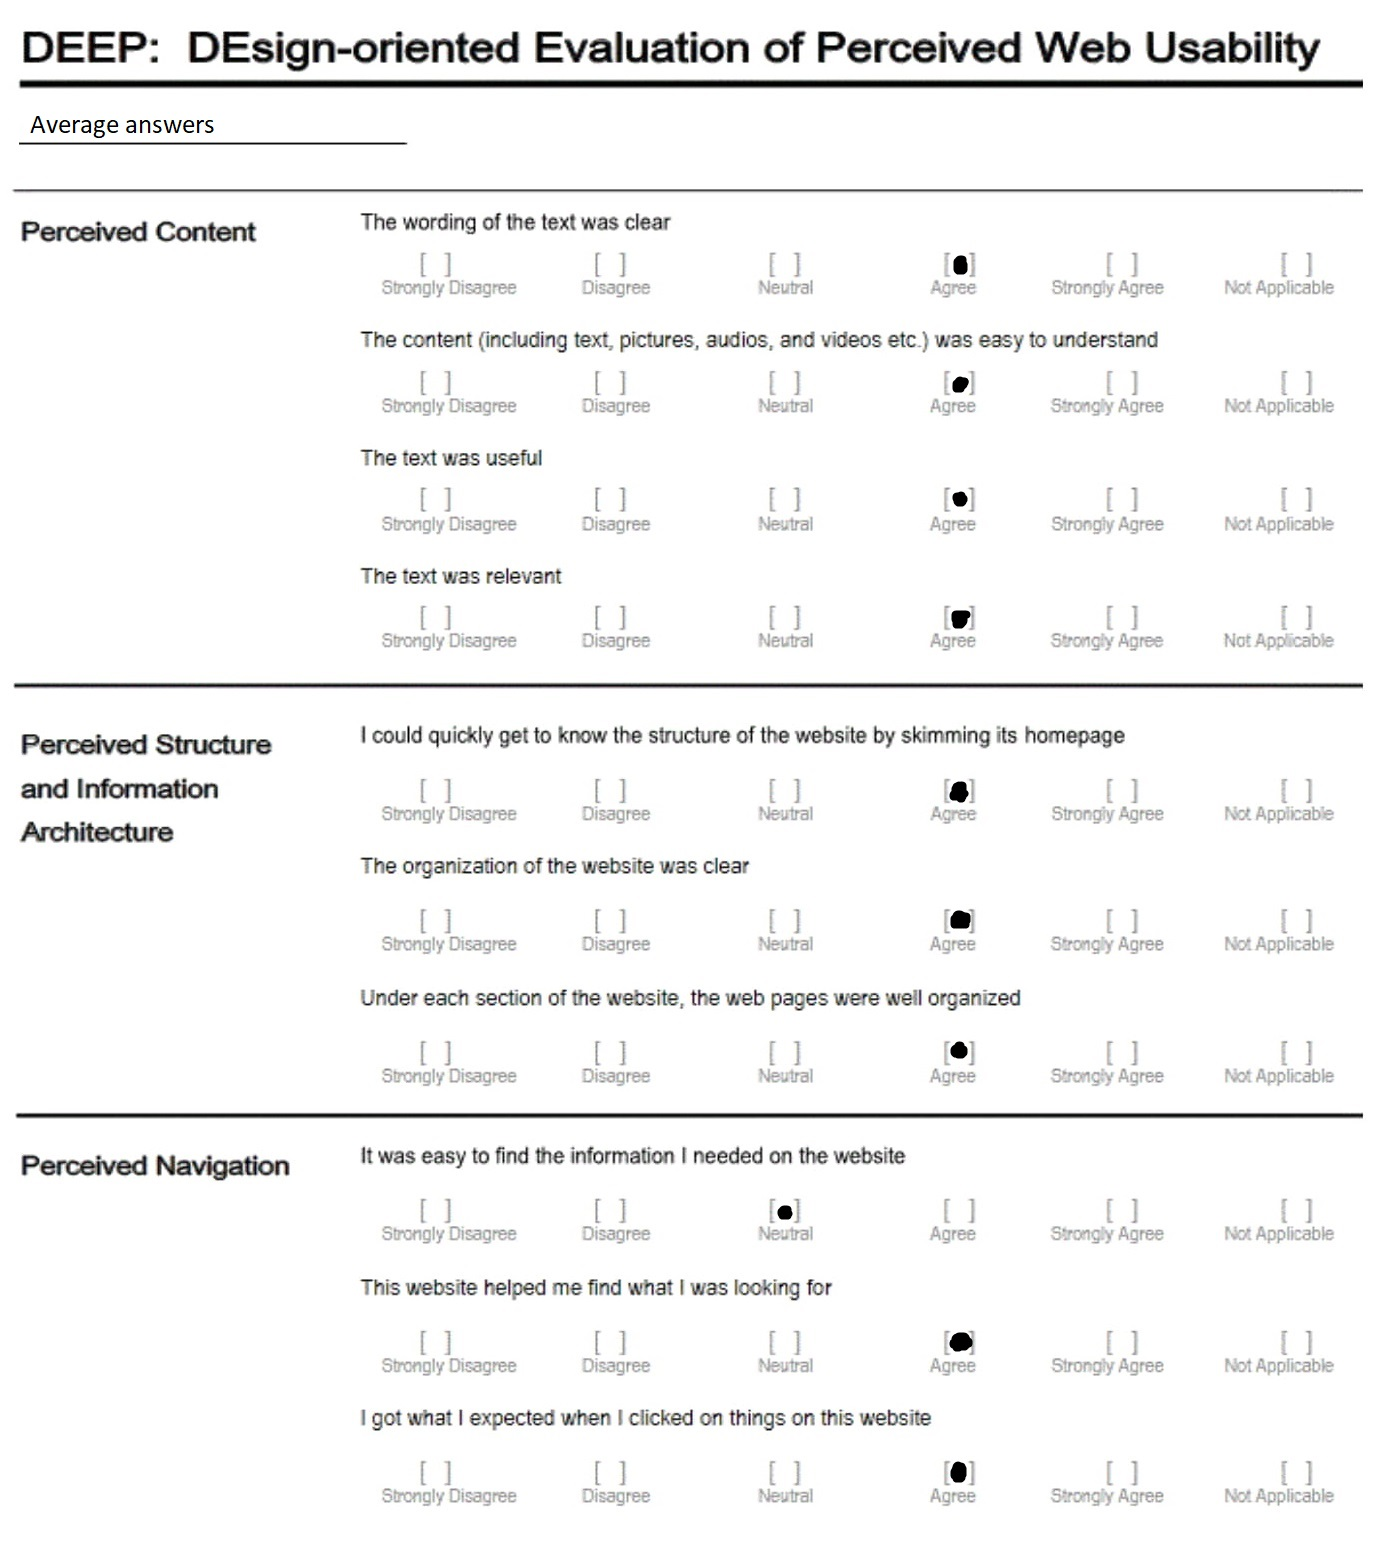
\includegraphics[width=1.09\textwidth]{Documents/postavg}}
\end{center}

The overall satisfaction of the users towards the site structure, information architecture, content and navigatation is good. The only thing to note is the ease with which the users find the information needed, that doesn't have a good evaluation.

% -----------------------------END------------------------------------- %